To achieve selective detection of histamine using an electrolyte-gated field-effect transistor (EG-FET), the functionalization of the gate electrode is essential. Without a dedicated sensing layer, the device lacks specificity and may respond to various interfering species. This section describes the modification of the gate with a histamine aptamers, enabling precise and reliable detection.

The detection of histamine turned out to be more complex than expected. The thiol and gold chemistry is a very simple chemistry, yet it needs some precautions to get successful results. The attachment of aptamers and PEG depends on many factors, including the roughness of the surface and the amount of contamination on the gold. In the case of the devices presented here, the surface is very smooth due to metal evaporation and rich in carbon contamination due to the long handling of the devices after fabrication and before functionalization and deposition of carbon nanotubes. XPS experiments have confirmed these hypotheses, showing a carbon contamination of 42\%, which is reduced to 18\% after 5 minutes of ozone treatment.
This solution is simple, inexpensive, and effective; the problem with the devices presented here is that functionalization must occur after deposition of the CNTs and the lipophilic membrane. This causes the CNTs to be deeply damaged by ozone. Figure \ref{fig:BeforeAfterClean} shows the normalized current of a device before (in red) and after (in blue) ozone treatment, following the standard protocol seen above, in which 40 transfer curves were collected consecutively over a period of one hour. It is evident how the operation of the device before cleaning mirrors the results in \ref{cap:chapter3}, while the operation after cleaning shows a current that decreases rapidly with time, \ie{} the platform is no longer stable. This result indicates that the membrane is not impermeable to ozone and does not protect the underlying CNTs. Further experiments were conducted by coating the channel with different substrates, such as polyimide and silicon, and none were able to sufficiently protect the CNTs.

\begin{figure}
    \centering
    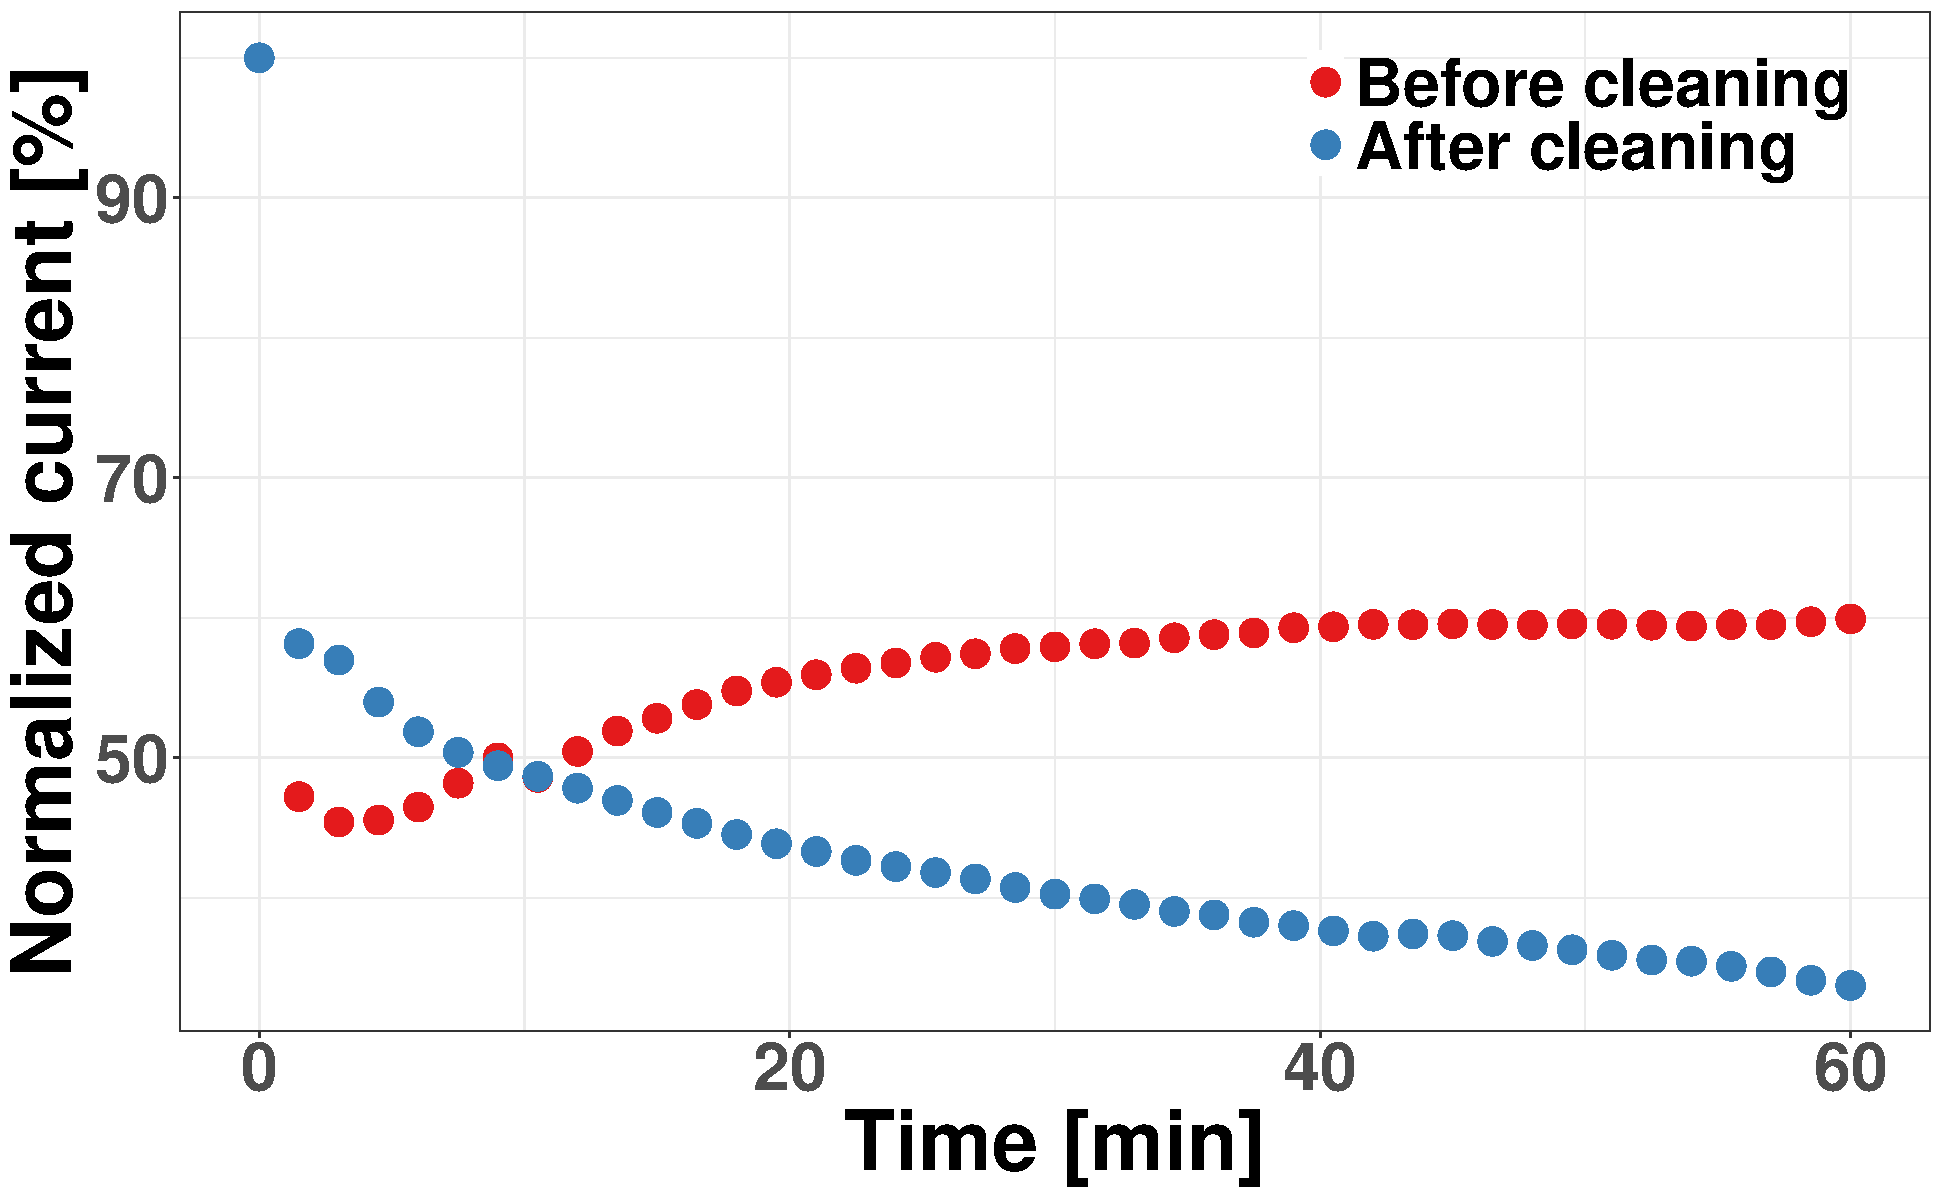
\includegraphics[width = 0.4\textwidth]{figures/chapter4/histamine/BeforeAfterClean.pdf}
    \caption{Normalized current measured using the standard protocol consisting of 40 consecutive transfer curve acquisitions over the span of one hour. The comparison between the current before (red) and after (blue) the ozone cleaning protocol reveals a clear degradation of device performance. Following ozone treatment, the device exhibits a continuous decrease in current, indicating that the cleaning process damages the CNTs. As a result, prior efforts toward stabilization are no longer valid and a different protocol must be found.}
    \label{fig:BeforeAfterClean}
\end{figure}

The second gate cleaning strategy tested was a chemical type of cleaning. Research showed that a very effective type of cleaning involved mixing \SI{50}{mM} \ce{KOH} and 25\% \ce{H2O2} \citep{fischerGold2009}; according to the authors of the paper, this technique is the one that finds the best compromise (it reconciles best) between deep cleaning of the electrodes and the least amount of damage caused. In figure \ref{fig:cleaningDamages}, on the other hand, you can see the damage caused by this technique on the thin film of fabricated devices where the gate has missing parts, corresponding to the effervescence of the solution. This effect can also be seen even when strongly diluting the two reagents, down to \SI{12.5}{mM} \ce{KOH} and 6.25\% \ce{H2O2}. Therefore, this strategy has to be discarded and an alternative solution has to be found.

The strategy adopted for the experiments shown below was to separate the gate from the signal-carrying component (channel) for separate cleaning.

\begin{figure}
    \centering
    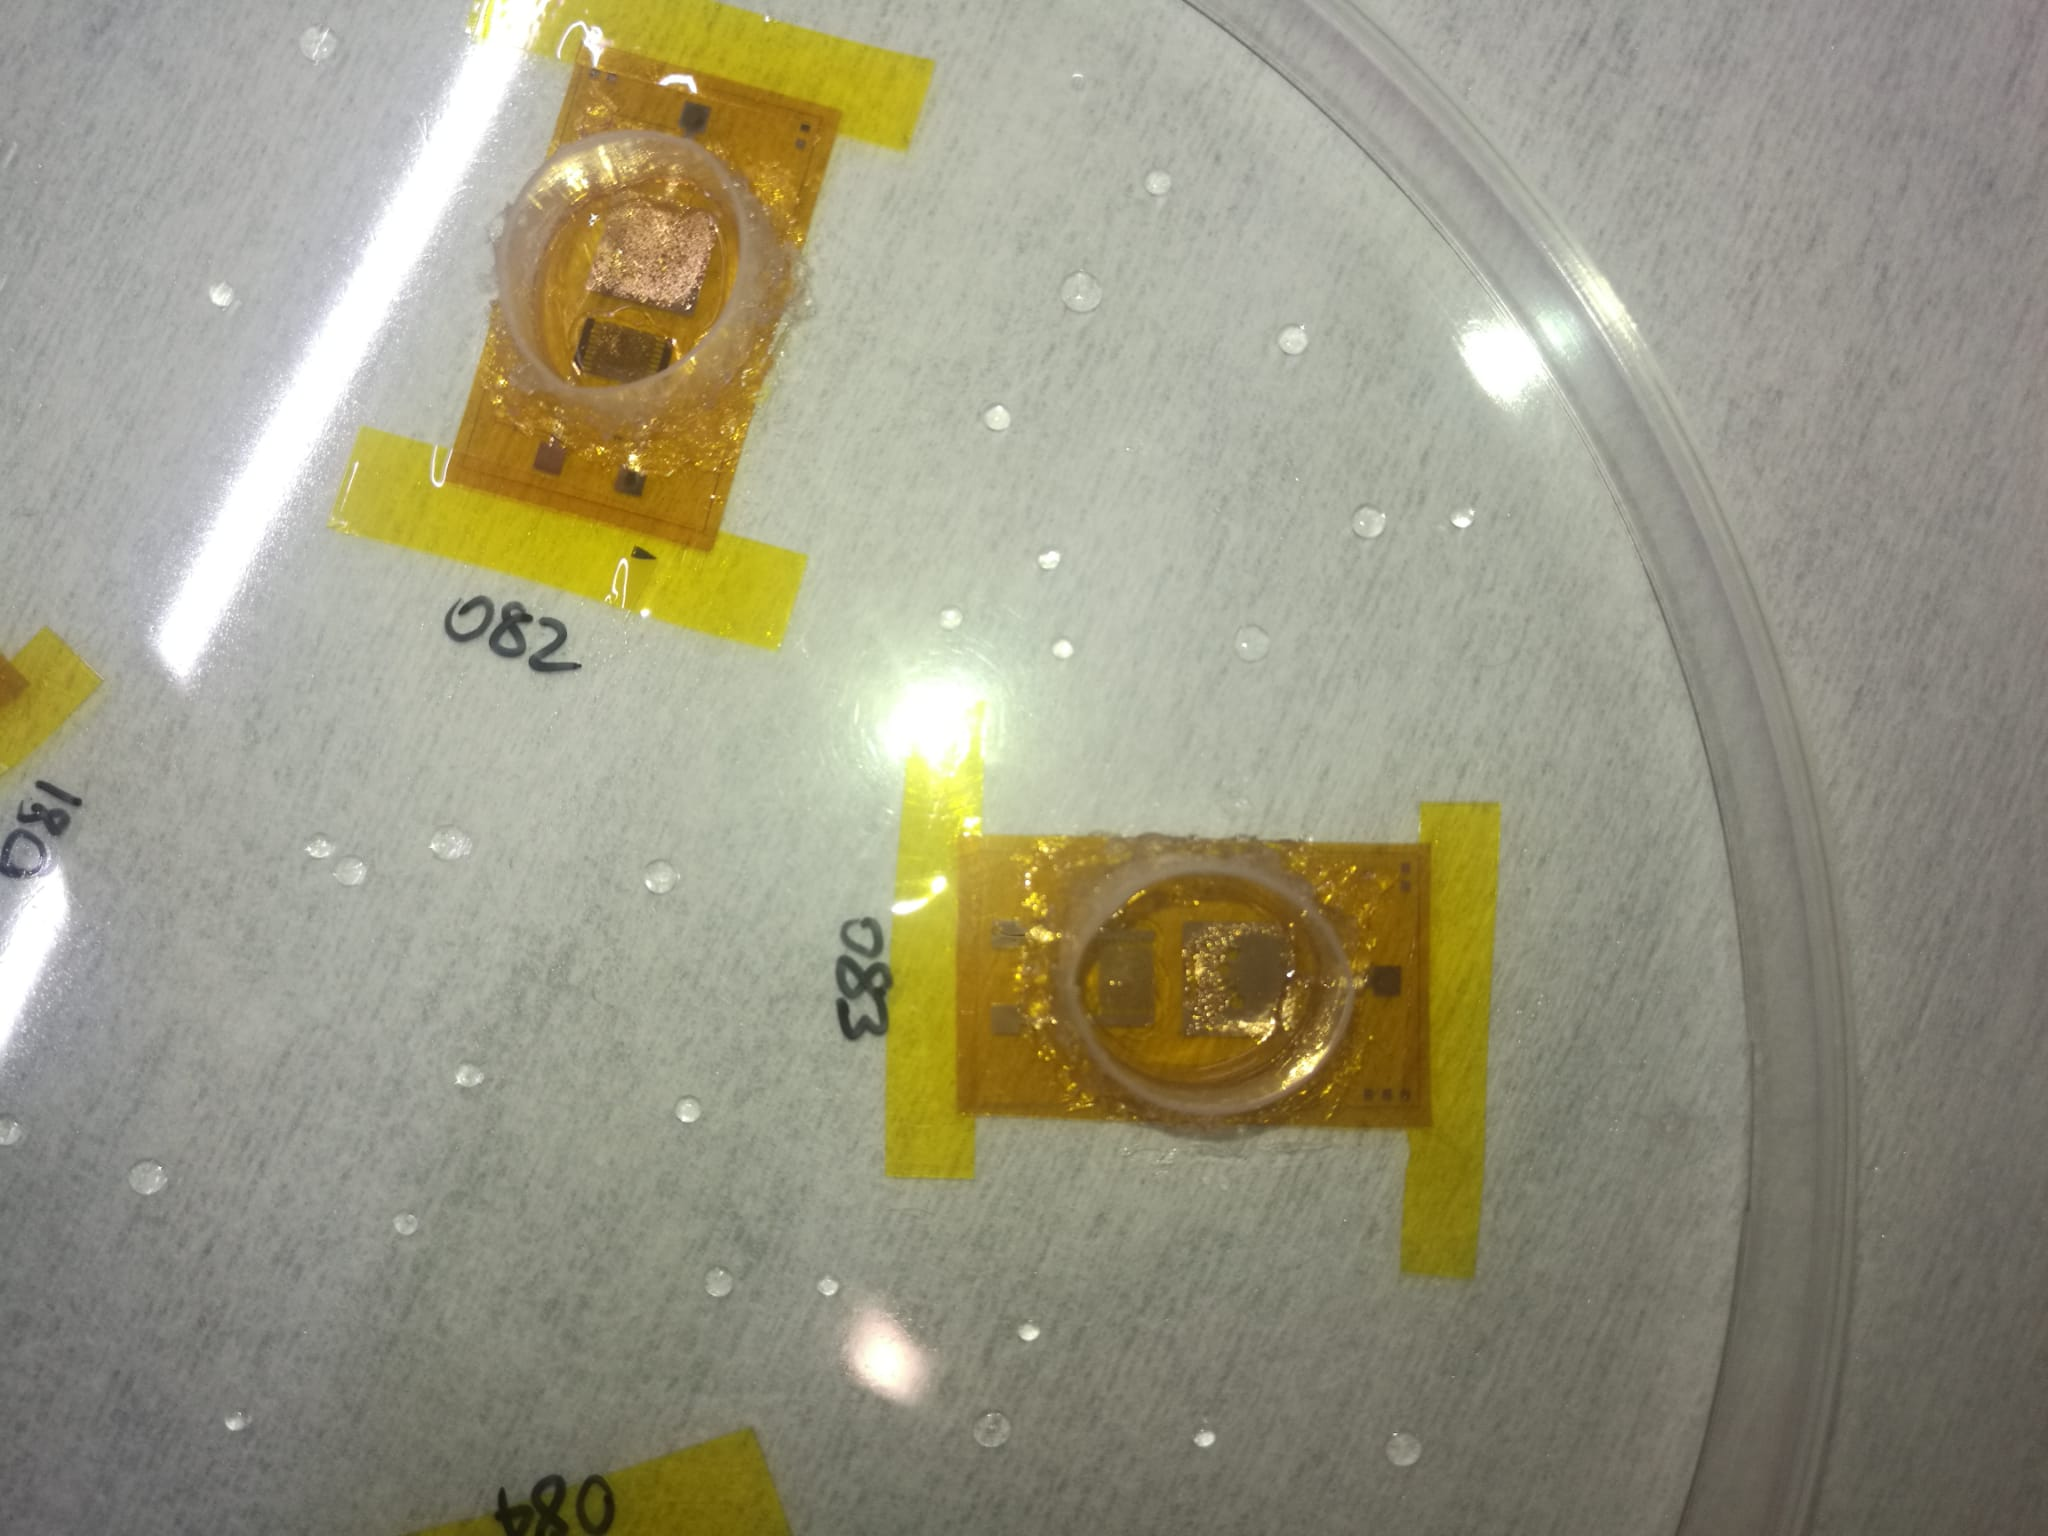
\includegraphics[width = 0.4\textwidth]{figures/chapter4/histamine/cleaningDamages.jpeg}
    \caption{Examples of damaged gates of two devices after treatment with \SI{50}{mM} \ce{KOH} and 25\% \ce{H2O2}, following the cleaning protocol described by \citet{heiskanenMonitoring2008}. While \citet{fischerGold2009} identified this method as the best compromise between cleaning efficacy and contained material damages, our results show significant degradation. The effervescence produced by the solution led to the delamination of the gold layer, particularly in areas where gas bubbles formed. These findings indicate that the protocol is incompatible with our devices, needing to search for an alternative cleaning strategy.}
    \label{fig:cleaningDamages}
\end{figure}

After cleaning, the functionalization was followed by electrochemical techniques, specifically cyclic voltammetry (CV). Figure \ref{fig:CVfunctionalization} shows that the current decreases and the redox peak shifts after each functionalization step. The effect is particularly noticeable after incubation with aptamers. This is even more pronounced after covering the entire surface with polyethylene glycol, which leads to the complete disappearance of the peak. This is due to the fact that with increasing surface coverage, the redox reaction can no longer take place, resulting in the disappearance of the peak. With this result, it was possible to confirm that the gate surface was properly functionalized and to proceed with the electrical characterization by collecting transfer and output characteristics, as well as chronoamperometric measurements.

\begin{figure}[hb]
    \centering
    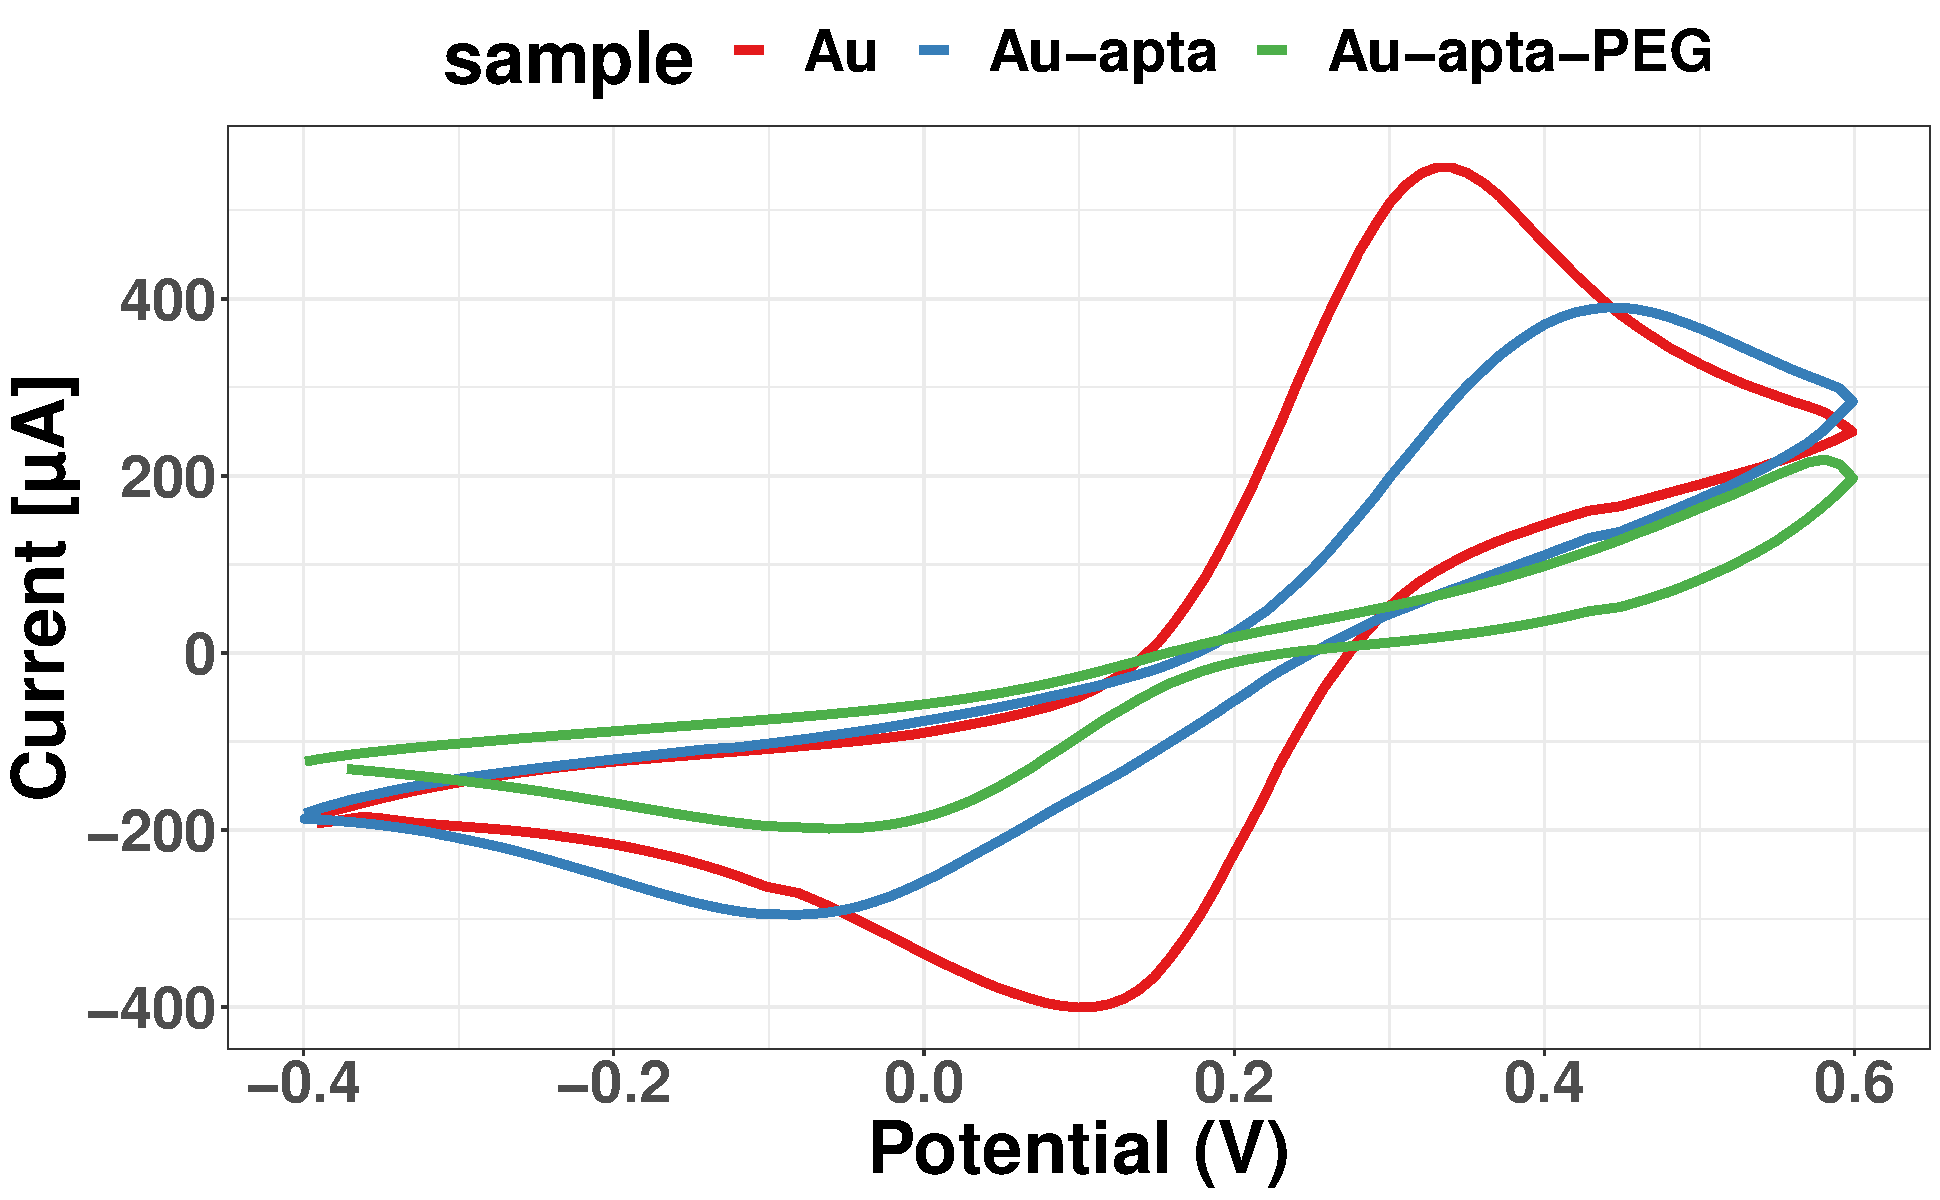
\includegraphics[width = 0.4\textwidth]{figures/chapter4/histamine/CV_functionalization.pdf}
    \caption{Cyclic voltammograms (CV) recorded after each stage of gate functionalization. The red curve corresponds to bare gold, the blue curve to gold functionalized with aptamers, and the green curve to gold modified with both aptamers and PEG. A progressive shift in peak position is observed following each modification step, accompanied by a decrease in peak current intensity. These effects indicate successful surface coverage: the shift in peak potential suggests changes in the interfacial electron transfer kinetics due to the presence of biomolecular layers, while the reduction in current intensity reflects the increasing barrier to charge transfer as the surface becomes more covered. The PEG layer, in particular, forms a dense, hydrophilic barrier that further hinders electron transfer, consistent with its role as a blocking agent.}
    \label{fig:CVfunctionalization}
\end{figure}

The measurement of the transfer curves was done with a first cycle of 40 curves (\SI{60}{\min}) necessary for the stabilization of the device; in fact, it can be observed that the corrected current, where the baseline has been removed, tends to \SI{0}{\uA}, which means that the linear fitting of the constant slope phase has been successful. Figure \ref{fig:normTransferHist} shows the variation of \ion{} over time, extracted from the transfer characteristics.
Second, 5 injections of histamine were made, increasing the concentration every 10 curves (\SI{15}{\min}). For the calibration curve (Figure \ref{fig:calTransferHist}), the mean and standard deviation of the last 5 \ion{} points of each concentration were calculated; the result is that histamine detection occurs linearly between \SIrange{0.01}{100}{\micro M}, with a sensitivity of \SI{0.15}{\uA \per decade}, with a coefficient of determination of 0.95.

\begin{figure}[htbp]
    \centering
    \subfloat[\ioncorr{}]{%
        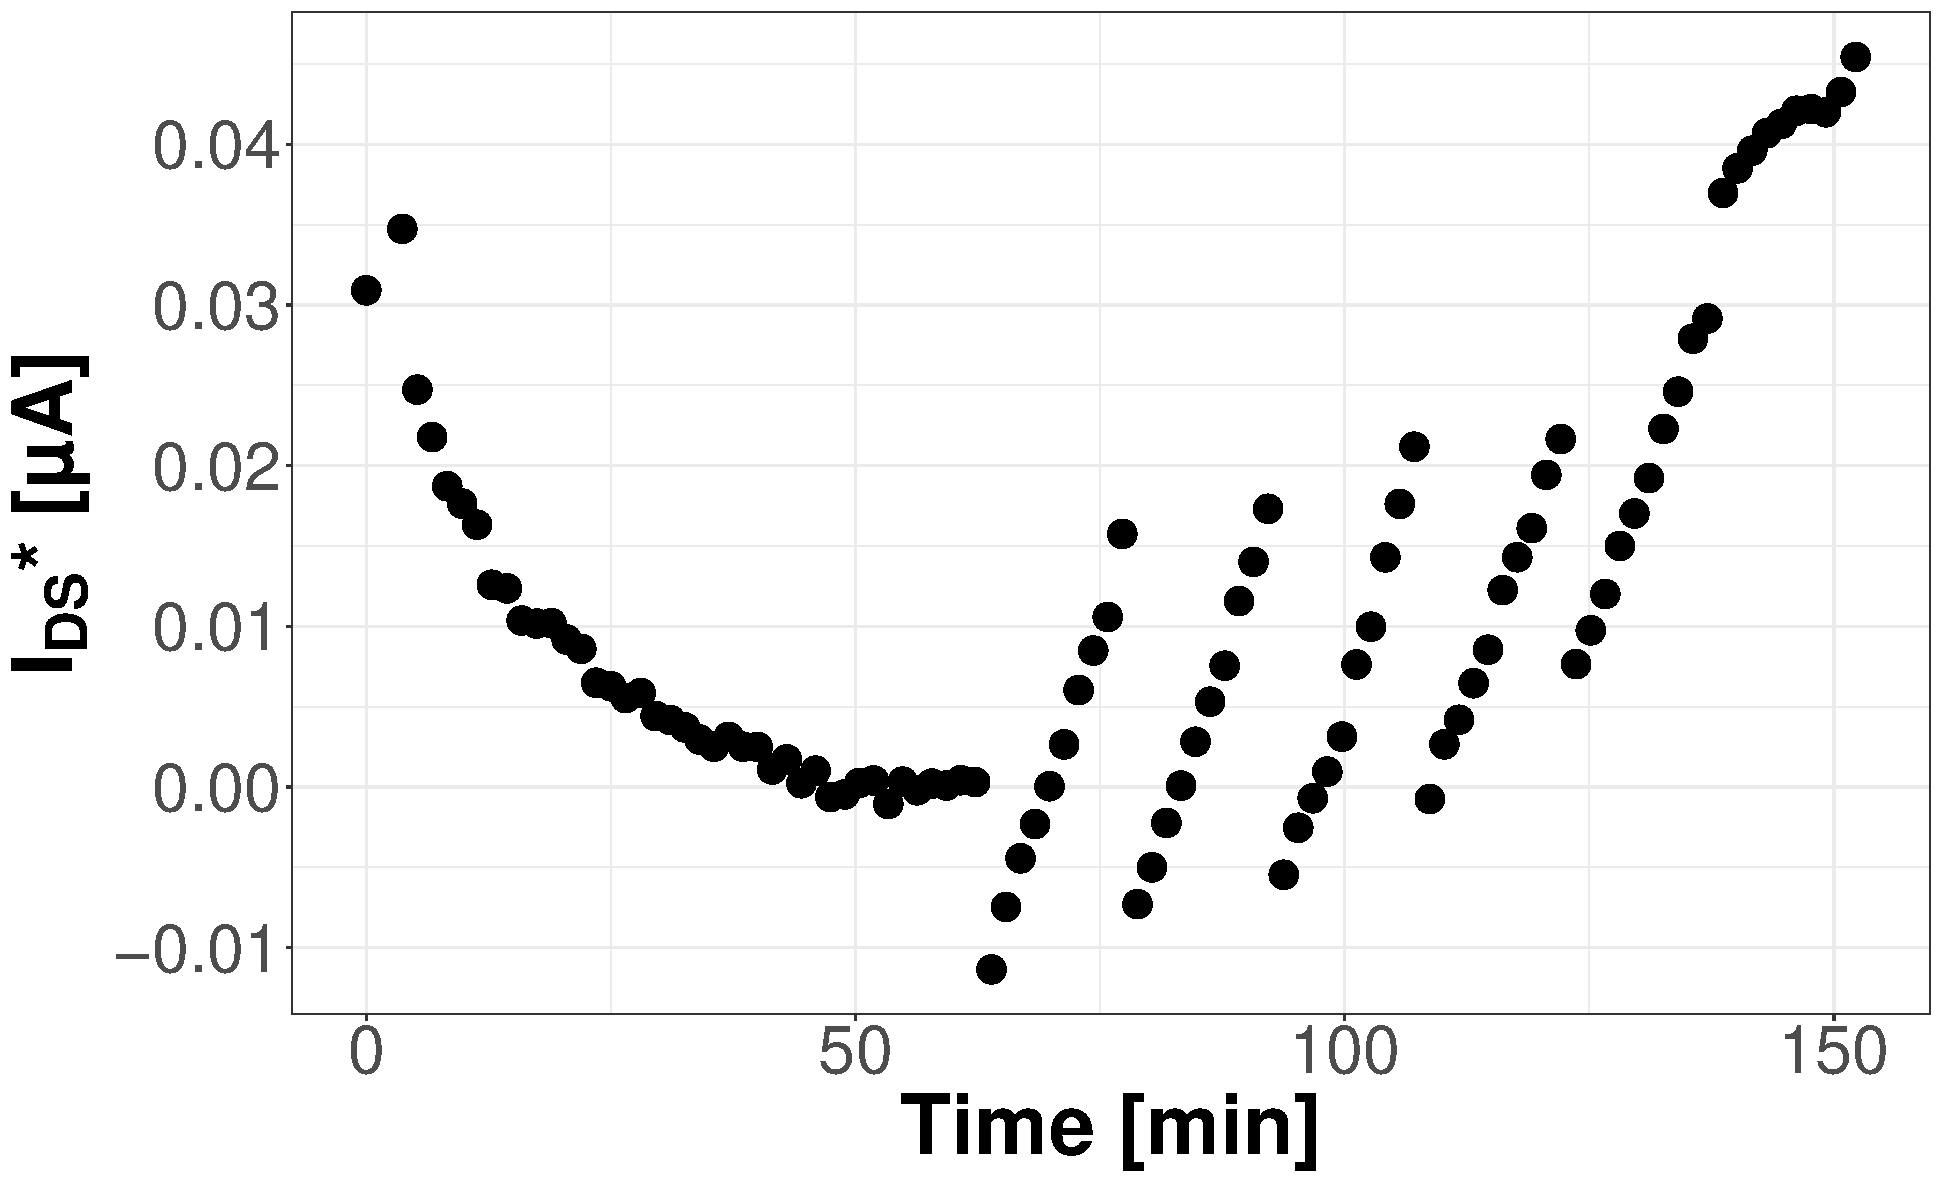
\includegraphics[width=0.4\textwidth]{figures/chapter4/histamine/correctedPlot-transfers.pdf}
        \label{fig:normTransferHist}
    }
    \quad
    \subfloat[Calibration curve]{%
        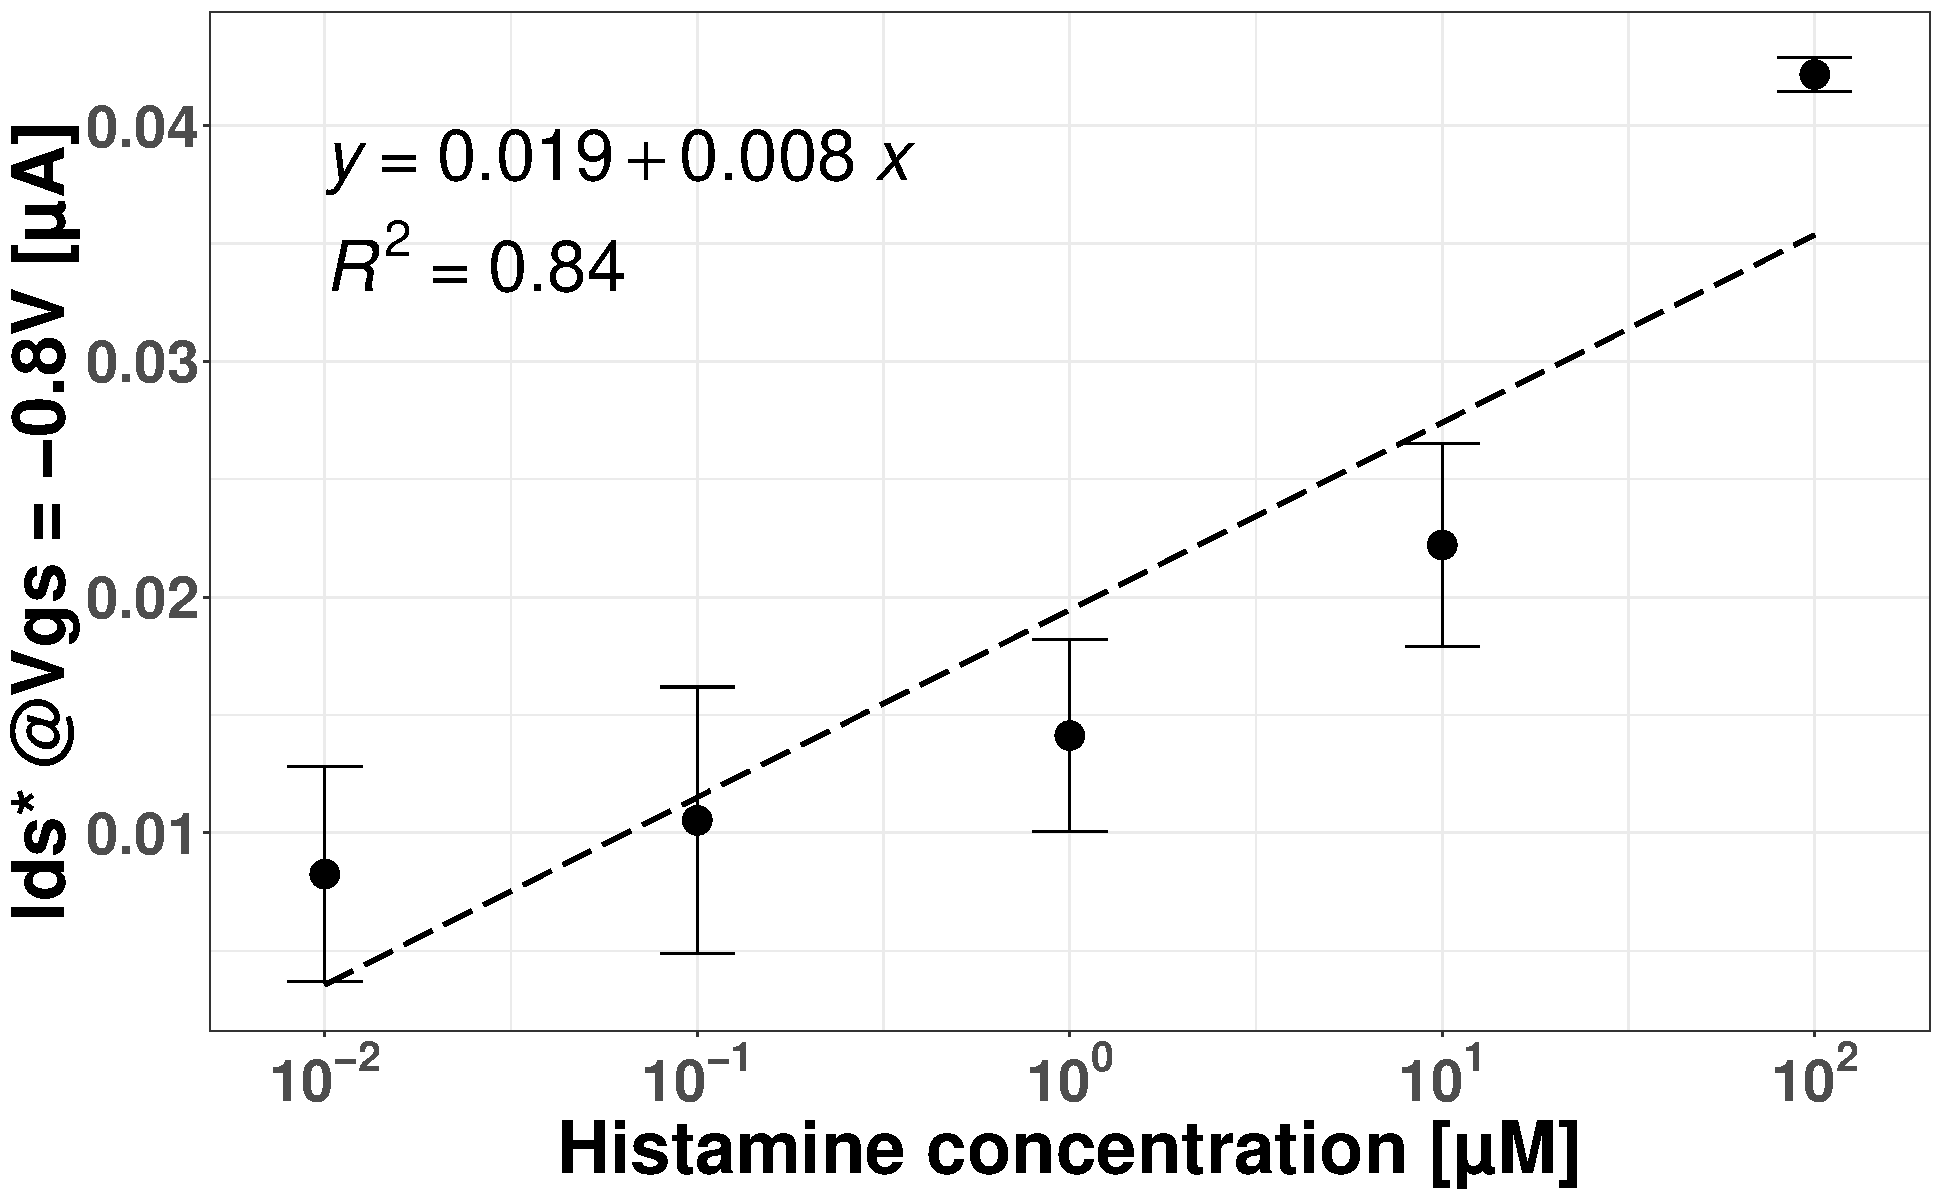
\includegraphics[width=0.4\textwidth]{figures/chapter4/histamine/calibrationPlot-transfers.pdf}
        \label{fig:calTransferHist}
    }
    \caption{Electrical characterization of the biosensor through transfer characteristics measurement.
        (a) \ioncorr{}. The \ion{} was extracted from each transfer curve and adjusted through baseline correction. Although individual injection events are clearly visible, this representation alone is not a reliable quantitative assessment. 
        (b) Calibration plot obtained by averaging the last five \ioncorr{} values after each injection. The sensor exhibits a linear response to histamine in the range of \SI{0.01}{\micro M} to \SI{100}{\micro M}, with a sensitivity of \SI{0.15}{\uA \per decade} and a coefficient of determination $R^2 = 0.95$.}
    \label{fig:HisTransfers}
\end{figure}

As in the case of the ammonium ion, measurements were made by fixing both \vds{} and \vgs{}. Figure \ref{fig:normChronoHist} shows the trend of the current at which the baseline was removed; as in the previous cases, the moments when the histamine-containing solution was injected appear. This graph gives us only a preliminary indication of the detection capability of the platform, so it is necessary to plot the calibration curve. As with the ammonium detection, the current measured over the last 5 minutes was averaged for each concentration tested. The result is shown in figure \ref{fig:calChronoHist}, where a linear trend is observed with a coefficient of determination of 0.96, but it is noted that the sensitivity of the sensor drops dramatically compared to the measurements made with transfer characteristics, being equal to \SI{0.028}{\uA \per decade}.

\begin{figure}[htbp]
    \centering
    \subfloat[\idscorr{}]{%
        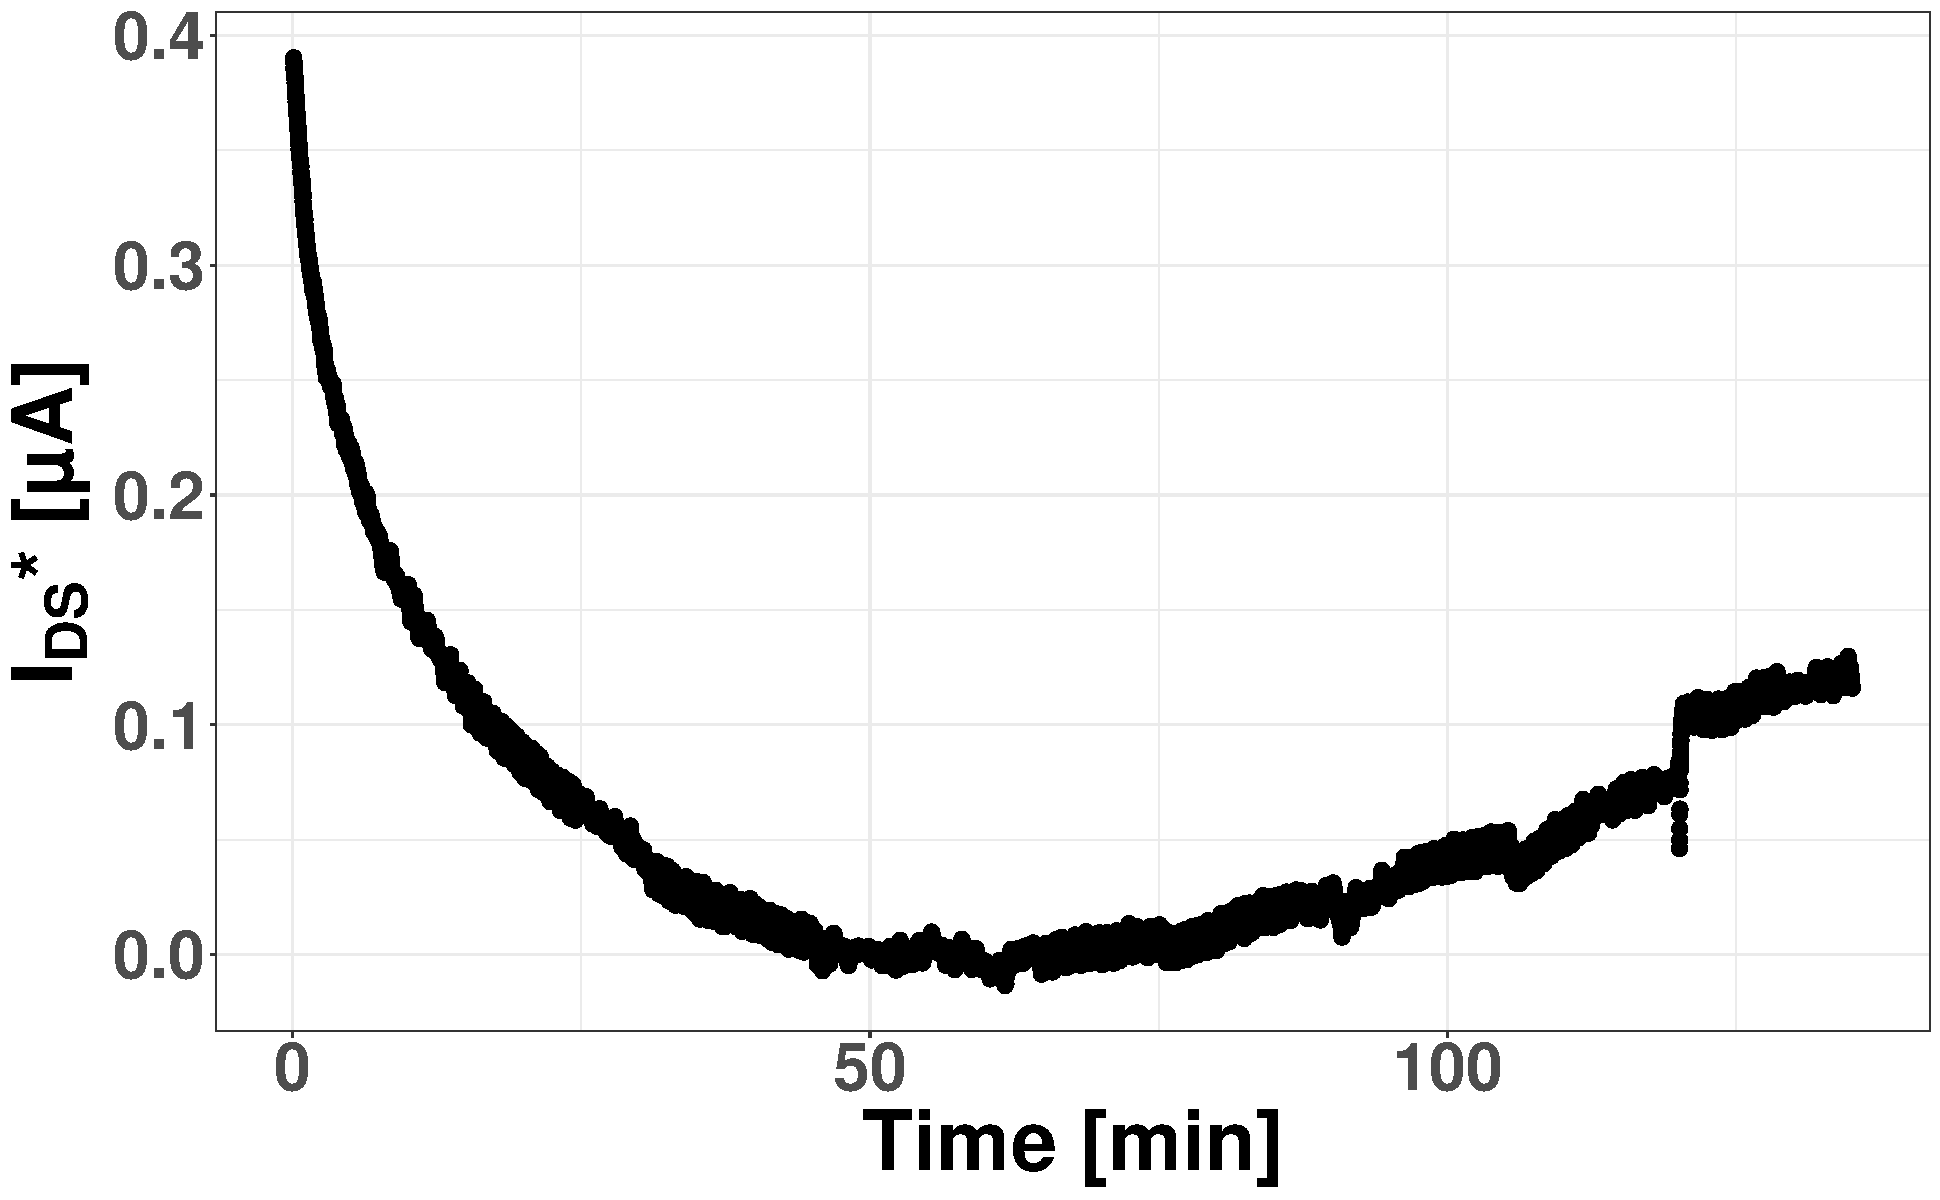
\includegraphics[width=0.4\textwidth]{figures/chapter4/histamine/correctedPlot-chronoamperometry.pdf}
        \label{fig:normChronoHist}
    }
    \quad
    \subfloat[Calibration curve]{%
        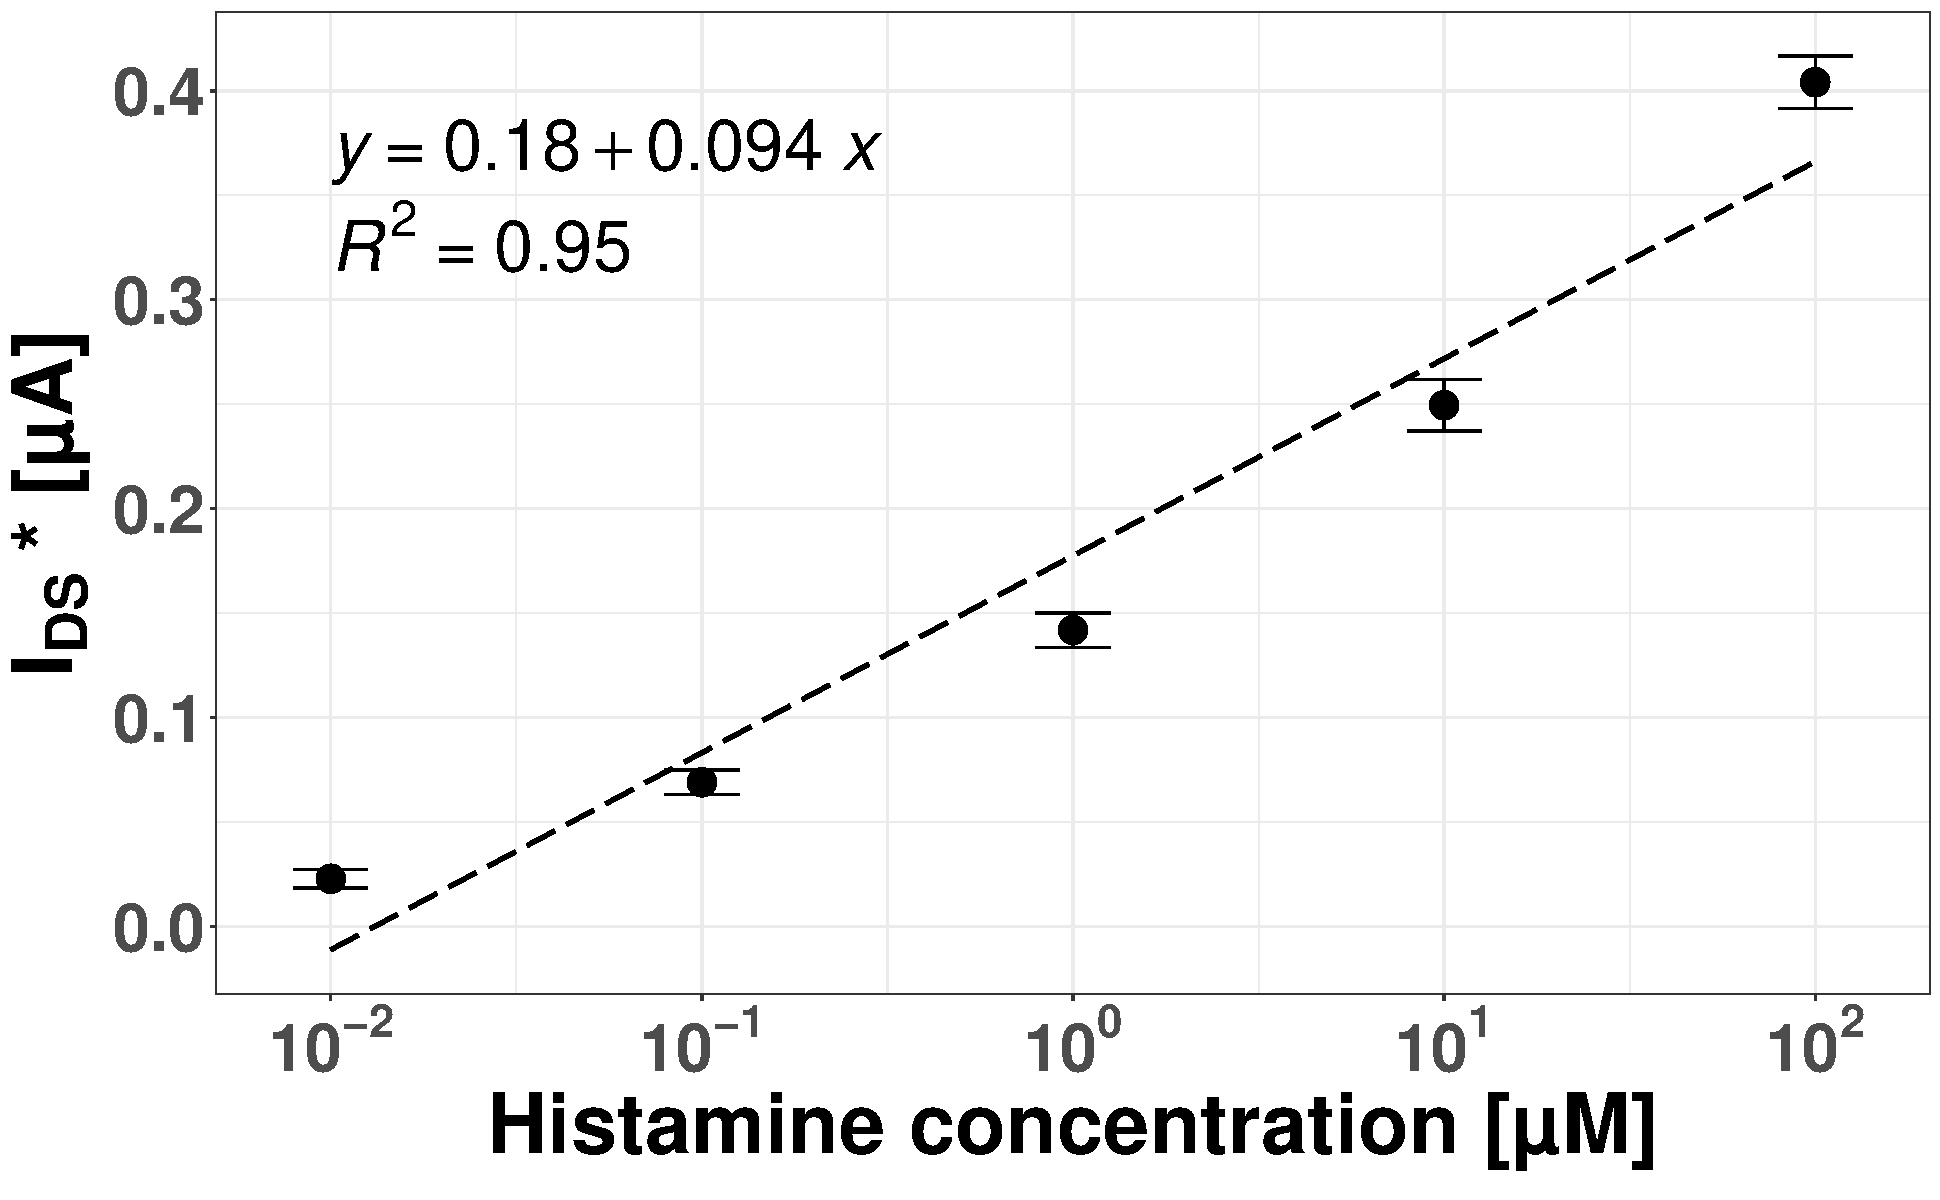
\includegraphics[width=0.4\textwidth]{figures/chapter4/histamine/calibrationPlot-chronoamperometry.pdf}
        \label{fig:calChronoHist}
    }
    \caption{Electrical characterization of the biosensor through chronoamperometric measurements.
    (a) \idscorr{} over time during chronoamperometric measurements for histamine detection. The injection events can be identified as small perturbations in the signal. 
    (b) Calibration curve obtained by averaging the final five points of the \idscorr{} for each tested concentration. The sensor exhibits a linear response with an \rsq{}$= 0.96$, although the sensitivity is significantly reduced compared to transfer-based measurements, reaching only \SI{0.028}{\uA \per decade}.
    }
    \label{fig:HisChrono}
\end{figure}


